\chapter{Bayesian Statistic}

\section{Statistic v.s. Probability}
Statistics focuses on real-life applications where the underlying distribution is often unknown. To address this, we use \textbf{statistical inference} to analyze observed data and estimate the unknown distribution. Rather than finding the exact distribution, we approximate it using models such as parametric (e.g., normal, exponential) or non-parametric approaches. Once a suitable model is chosen, probability laws help us make predictions and draw conclusions, though these approximations involve assumptions and uncertainties.  

Now, let's move on to our first topic in statistics: 

\section{Bayesian Statistics}

\subsection{Introduction}
In the probability course, we learned Bayes' Rule \href{https://ryanc.wtf/files/ENGG2760.pdf#page=14}{ENGG2760: Theorem 3.2.1}, which helps us calculate conditional probabilities and, at times, update our beliefs based on new evidence.

And it turns out that one of the statistical inferences we use is based on Bayes' rule, namely Bayesian statistical inference. In Bayesian statistical inference, we: (1) assign prior probabilities to parameters; (2) observe data; and (3) update probabilities via Bayes' rule:
\[
  \underbrace{f_{\Theta \vert X} (\theta \vert x)}_{\text{Posterior}} = \dfrac{\overbrace{f_{\Theta} (\theta)}^{\text{Prior}} \overbrace{f_{X \vert \Theta} (x \vert \theta)}^{\text{Observation}}}{f_X (x)}
\]
Here we have both the posterior and prior probabilities of the parameters \(\theta\)  and observations \(x\).  

We have four variations of the Bayes' rule shown above.

\begin{table}[H]
  \centering
  \begin{tabular}{c|c}
      \toprule
      Condition & Bayes' rule  \\
    \midrule
      \(\Theta\) discrete, \(X\) discrete & \(p_{\Theta \vert X} (\theta \vert x) = \dfrac{p_{\Theta} (\theta) p_{X \vert \Theta} (x \vert \theta)}{\sum_{\theta^{\prime}} p_{\Theta} (\theta^{\prime}) p_{X \vert \Theta} (x \vert \theta^{\prime})}\)  \\
      \(\Theta\) discrete, \(X\) continuous & \(p_{\Theta \vert X} (\theta \vert x) = \dfrac{p_{\Theta} (\theta) f_{X \vert \Theta} (x \vert \theta)}{\sum_{\theta^{\prime}} p_{\Theta} (\theta^{\prime}) f_{X \vert \Theta} (x \vert \theta^{\prime})}\)  \\
      \(\Theta\) continuous, \(X\) discrete & \(f_{\Theta \vert X} (\theta \vert x) = \dfrac{f_{\Theta} (\theta) p_{X \vert \Theta} (x \vert \theta)}{\int f_{\Theta} (\theta^{\prime}) p_{X \vert \Theta} (x \vert \theta^{\prime})}\)  \\
      \(\Theta\) continuous, \(X\) continuous & \(f_{\Theta \vert X} (\theta \vert x) = \dfrac{f_{\Theta} (\theta) f_{X \vert \Theta} (x \vert \theta)}{\int f_{\Theta} (\theta^{\prime}) f_{X \vert \Theta} (x \vert \theta^{\prime})}\)  \\
      \bottomrule
  \end{tabular}
\end{table}

We can use \(Z(x)\) to denote the denominator for both discrete and continuous cases. It depends only on the observed data \(x\).

\begin{eg}[Probability Review]
  We flip a coin. How likely is it to get 2 heads in 3 coin flips if the probability of heads is \(p\), where \(p\) could be 0.5, 0.7, and 1? 
  
  Also, use the Central Limit Theorem to estimate the probability of at least 200 heads in 300 coin flips.

  \textbf{Solution:} 
  \[
    \mathbb{P}(H = 2) = \binom{3}{2} p^2(1 - p)
  \]
  \(p = 0.5: \mathbb{P}(H = 2) = \binom{3}{2} \times 0.5^2 \times 0.5 = 0.375\)

  \(p = 0.7: \mathbb{P}(H = 2) = \binom{3}{2} \times 0.7^2 \times 0.3 = 0.441\)

  \(p = 1: \mathbb{P}(H = 2) = \binom{3}{2} \times 1^2 \times 0 = 0\)

  For the probability of at least 200 heads in 300 coin-flips, 
  \[
    \text{H} \sim \text{Binomial}(300, p),\quad \mu = 300p,\quad \sigma = \sqrt{300p(1 - p)}
  \]
  \(p = 0.5: \mu = 150, \sigma = 8.66\)

  \(
  \begin{aligned}
    \mathbb{P}(H \geq 200) &= \mathbb{P}(\dfrac{H - 150}{8.66} \geq \dfrac{200 - 150}{8.66}) \\
    &= \mathbb{P}(z \geq 5.77) \\
    &\approx 0
  \end{aligned}
  \) 

  \(p = 0.7: \mu = 210, \sigma = 7.94\)

  \(
  \begin{aligned}
    \mathbb{P}(H \geq 200) &= \mathbb{P}(\dfrac{H - 210}{7.94} \geq \dfrac{200 - 210}{7.94}) \\
    &= \mathbb{P}(z \geq -1.26) \\
    &= \varPhi (1.26) \\
    &= 0.896
  \end{aligned}
  \) 
  
\end{eg}

Again, we flip a coin three times and get two heads. You are told that there are three types of coins with different priors, but you don’t know which coin you are flipping. It is obvious that the first coin flip will affect your belief (prior) about which coin you have. For example, if you see 100 heads out of 100 flips, you might strongly believe that both sides of the coin are heads. But to what extent does each flip influence your belief? This brings us to the problem of statistics.

\begin{eg}
  A coin can be one of three types:

  1. A fair coin \(\theta = 1\) with one head and one tail – 90\%

  2. A coin \(\theta = 2\) with both sides as heads – 5\%
  
  3. A coin \(\theta = 3\) with both sides as tails – 5\%

  Now, you flip a head without knowing which coin you have. How should you update your belief (priors)?

  \textbf{Solution:} 

  \(
  \begin{aligned}
    \mathbb{P}(\theta = 1 \vert H_1) &= \dfrac{\mathbb{P}(H_1 \vert \theta = 1)\mathbb{P}(\theta = 1)}{Z(H_1)} = \dfrac{0.5 \times 0.9}{Z(H_1)} = \dfrac{0.45}{Z(H_1)} \\
    \mathbb{P}(\theta = 2 \vert H_1) &= \dfrac{\mathbb{P}(H_1 \vert \theta = 2)\mathbb{P}(\theta = 2)}{Z(H_1)} = \dfrac{1 \times 0.05}{Z(H_1)} = \dfrac{0.05}{Z(H_1)} \\
    \mathbb{P}(\theta = 3 \vert H_1) &= 0 \\
  \end{aligned}
  \) 

  Then we have \(\mathbb{P}(H_1) = Z(H_1) = 0.45 + 0.05 + 0 = 0.5\) 
  \[
    \mathbb{P}(\theta = 1 \vert H_1) = \dfrac{0.45}{Z(H_1)} = 0.9 \quad \mathbb{P}(\theta = 1 \vert H_1) = \dfrac{0.05}{Z(H_1)} = 0.1 \quad \mathbb{P}(\theta = 1 \vert H_1) = 0
  \]

  From this, we can update our belief, which we can then use to further readjust our belief if the second flip also results in a head. 

  \(
  \begin{aligned}
    \mathbb{P}(\theta = 1 \vert H_2 H_1) &= \dfrac{\mathbb{P}(H_2 \vert \theta = 1, H_1)\mathbb{P}(\theta = 1 \vert H_1)}{Z(H_2, H_1)} = \dfrac{0.5 \times 0.9}{Z(H_2, H_1)} = \dfrac{0.45}{Z(H_2, H_1)} \\
    \mathbb{P}(\theta = 2 \vert H_2 H_1) &= \dfrac{\mathbb{P}(H_2 \vert \theta = 2, H_1)\mathbb{P}(\theta = 2 \vert H_1)}{Z(H_2, H_1)} = \dfrac{1 \times 0.1}{Z(H_2, H_1)} = \dfrac{0.1}{Z(H_2, H_1)} \\
    \mathbb{P}(\theta = 3 \vert H_2 H_1) &= 0 \\
  \end{aligned}
  \) 

  Then we have \(\mathbb{P}(H_2 H_1) = Z(H_2 H_1) = 0.45 + 0.01 + 0 = 0.55\) 
  \[
    \mathbb{P}(\theta = 1 \vert H_2 H_1) = \dfrac{0.45}{Z(H_2 H_1)} = 0.82 \quad \mathbb{P}(\theta = 1 \vert H_2 H_1) = \dfrac{0.1}{Z(H_2 H_1)} = 0.18 \quad \mathbb{P}(\theta = 1 \vert H_2 H_1) = 0
  \]
\end{eg}

We also have Bayes's rule for multiple random variables:
\[
  \begin{aligned}
    f_{\Theta \vert X_1, \cdots, X_n} (\theta \vert x_1, \cdots, x_n) &= \dfrac{f_{X_1, \cdots, X_n \vert \Theta} (x_1, \cdots, x_n \vert \theta) f_{\Theta} (\theta)}{Z(x_1, \cdots, x_n)} \\
    &\propto f_{X_1, \cdots, X_n \vert \Theta} (x_1, \cdots, x_n \vert \theta) f_{\Theta} (\theta) \\ 
    &= \underbrace{f_{X_1 \vert \Theta} (x_1 \vert \theta) \cdots f_{X_n  \vert \Theta(x_n \vert \theta)}}_{\text{product of likelihood}} \underbrace{f_{\Theta} (\theta)}_{\text{prior}}
  \end{aligned}
\]
if \(X_1, \cdots, X_n\) are independent given \(\Theta\).  

% L01 finished
\subsection{Bayesian Statistical Inference}
For Bayesian statistics, we have only one formula: Bayes’s rule: 
\[
  \underbrace{f_{\Theta \vert X} (\theta \vert x)}_{\text{posterior}} \propto \underbrace{f_{X \vert \Theta} (x \vert \theta)}_{\text{likelihood}} \underbrace{f_{\Theta} (\theta)}_{\text{prior}}
\]

We have some prior knowledge, and after observing something, we can use the prior and likelihood to update our belief, which gives us the posterior. This posterior can later serve as the prior for another observation, allowing us to continuously update our belief throughout the observation process.

\begin{eg}
  Romeo is waiting for Juliet on their first date. He wants to estimate how long he will have to wait for her. Given that Romeo has some prior dating experience, he already has some prior knowledge about how late girls tend to be.
  
  Girl A - \(X \sim \text{Uniform}(0, 0.3)\); 
  
  Girl B - \(X \sim \text{Uniform}(0, 0.8)\); 

  Girl C - \(X \sim \text{Uniform}(0, 0.6)\), 

  where the uniform random variable shows the range of lateness. For example, for girl A, she will be late between the dating time and the dating time plus 0.3 hours. Then, how could you use Bayesian statistics to estimate the waiting time for Romeo's new girlfriend? 

  \textbf{Solution:} 
  Here we can set up the uniform random variable \(\text{Uniform}(0, \Theta)\), where \(\Theta\) depends on the girls' decision. Then what we need to find is the \(\theta\) for Juliet. We can then have 
  \[
    f_{X \vert \Theta}(x \vert \theta) = \begin{dcases}
      \frac{1}{\theta}, &\text{ if } 0 \leq x \leq \theta ;\\
      0, &\text{ otherwise} .
    \end{dcases}
  \]

  In Romeo's model, \(\theta\) is also a uniform random variable \(\theta \sim \text{Uniform}(0, 1)\), where \(X \sim \text{Uniform}(0, \Theta)\). Given that on their first date, Juliet arrived \(\frac{1}{2}\) hours late, we have 
  \[
    f_{\Theta \vert X} (\theta \vert \dfrac{1}{2}) \propto f_\Theta (\theta) f_{X \vert \Theta}(\dfrac{1}{2} \vert \theta) = \dfrac{1}{\theta}
  \]
  Here we have the prior \(f_\Theta(\theta) = 1\) if \(0 \leq \theta \leq 1\), and the likelihood \(f_{X \vert \Theta} (\frac{1}{2} \vert \theta) = \frac{1}{\theta}\) if \(\frac{1}{2} \leq \theta \leq 1\). Keep in mind that the prior comes from Romeo's model, where he has never dated a girl who is late for more than 1 hour, and it may not be valid if \(\theta > 1\), which shows the limitation of Bayesian statistics. Also, the observation (likelihood) shows the probability of Juliet arriving precisely at (or within a very small interval around) time plus 0.5. Therefore, we have \(\theta \geq \frac{1}{2}\). 

  For the integral to be equal to 1, we need to find the constant term. This can be found using calculus: 
  \[
    \int_\frac{1}{2} ^1 \dfrac{1}{\theta} d \theta= \ln \theta \Big|_{\frac{1}{2}}^1 = \ln 2 \Longrightarrow f_{\Theta \vert X} (\theta \vert \dfrac{1}{2}) = \dfrac{1}{\theta \ln 2}
  \]

  \begin{minipage}{0.5\textwidth}
    Here we have \(\theta < \frac{1}{2} = 0\) because from the data, we know that \(\theta \geq \frac{1}{2}\), which means the lateness parameter is at least \(\frac{1}{2}\), so it is not possible for Juliet to arrive between the dating time and dating time plus 0.5. We also have \(\theta > 1 = 0\) because from Romeo's prior knowledge, he knows that a girl would not be later than 1 hour.
  \end{minipage}
  \begin{minipage}{0.5\textwidth}
    \centering
    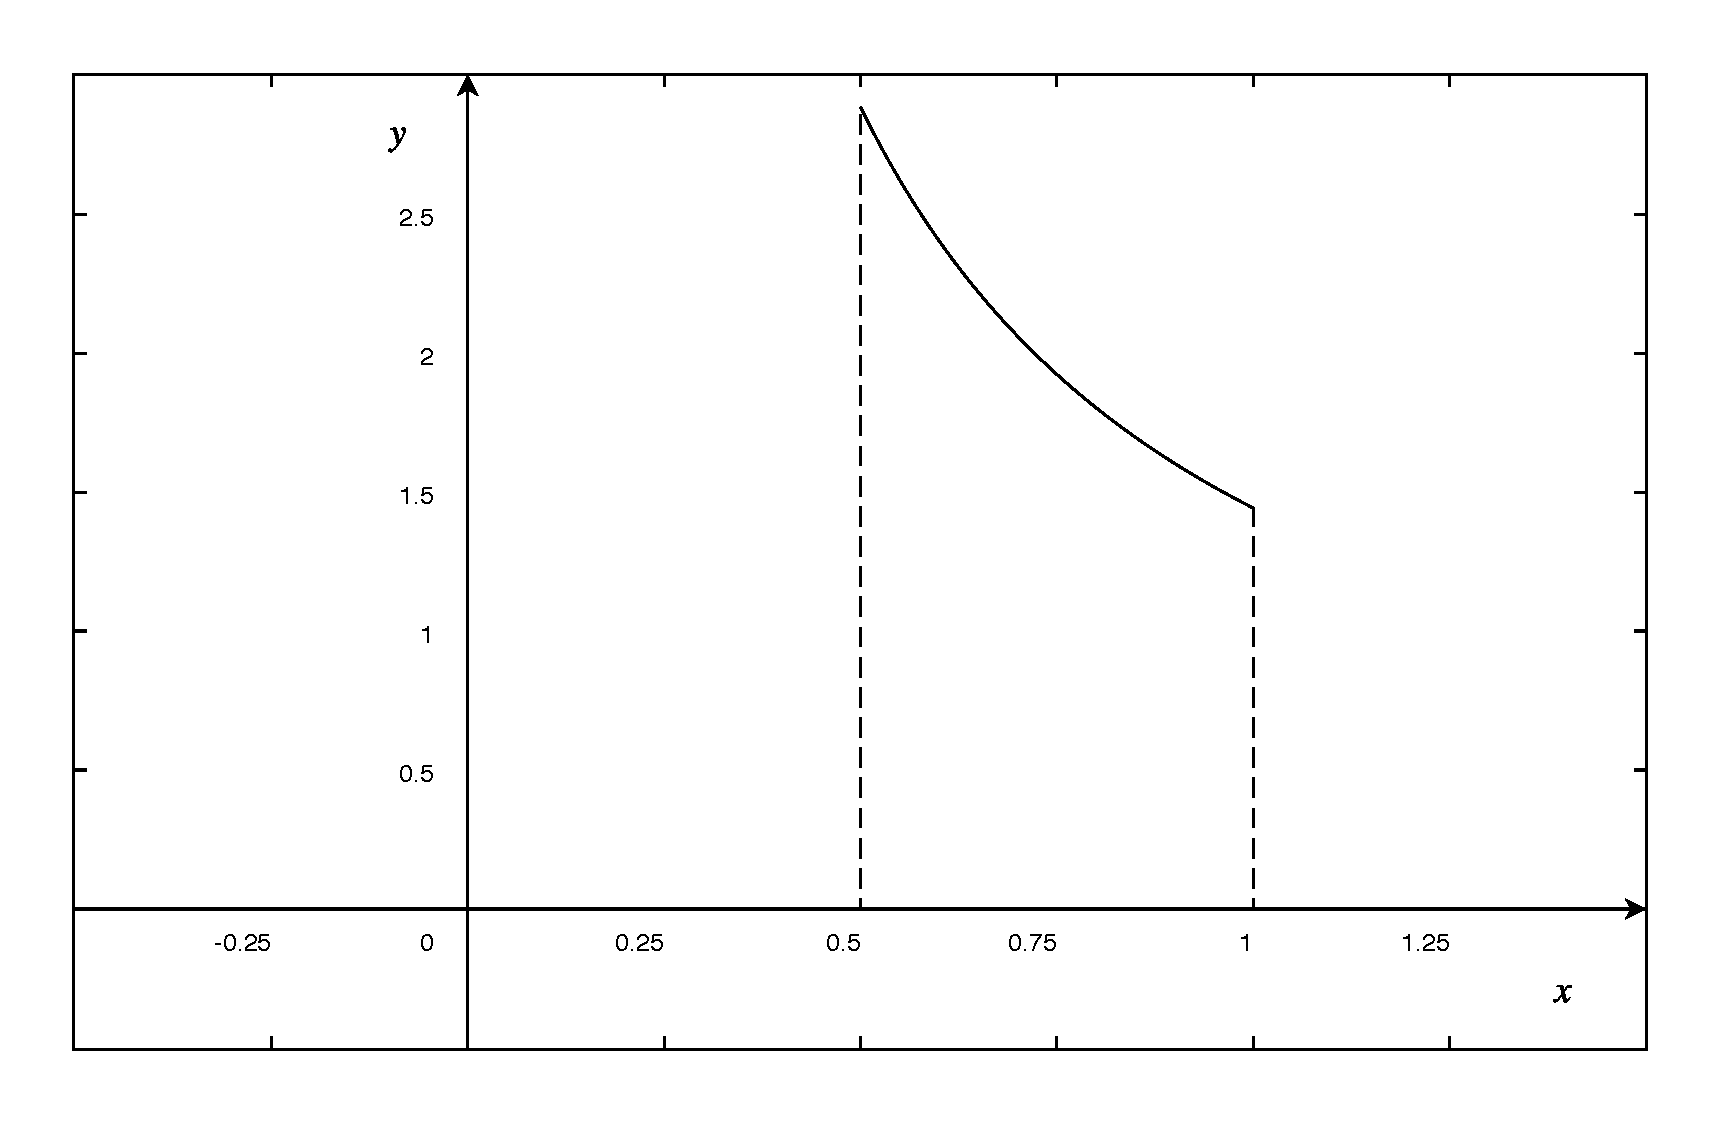
\includegraphics[width=0.8\textwidth]{Figures/Romeo_model.pdf}
  \end{minipage}

  On their second date, Juliet arrived \(\frac{1}{4}\) hours late. We then need to readjust the prior based on the previous model to find the new posterior.
  \[
    f_{\Theta \vert X_1, X_2} \left(\theta \Big| \dfrac{1}{2}, \dfrac{1}{4}\right) \propto f_{\Theta \vert X_1} \left(\theta \Big| \dfrac{1}{2}\right) f_{X_2 \vert \Theta, X_1}\left(\dfrac{1}{4} \Big| \theta, \frac{1}{2}\right)
  \]
  Here, since \(X_1\) and \(X_2\) are independent, we can discard \(X_1\) in the calculation.
  \[
    f_{\Theta \vert X_1, X_2} \left(\theta \Big| \dfrac{1}{2}, \dfrac{1}{4}\right) \propto f_{\Theta \vert X_1} \left(\theta \Big| \dfrac{1}{2}\right) f_{X_2 \vert \Theta}\left(\dfrac{1}{4} \Big| \theta\right) = \dfrac{1}{\theta \ln 2} \times \dfrac{1}{\theta} = \dfrac{1}{\theta^{2} \ln{(2)}} \propto \dfrac{1}{\theta^2}
  \]
  The same as above, we have \(f_{X_2 \vert \Theta} (\frac{1}{4} \vert \theta) = \frac{1}{\theta}\) since it is not possible for the lateness to be less than \(\frac{1}{4}\) hours. Also, given the prior as calculated in the first part, we have \(f_{\Theta \vert X_1} (\theta \vert \frac{1}{2}) = \frac{1}{\theta \ln 2}\) if \(\frac{1}{2} \leq \theta \leq 1\).

  For the integral to be equal to 1, we need to find the constant term. This can be found using calculus: 
  \[
    \int_\frac{1}{2} ^1 \dfrac{1}{\theta^2} d \theta = 1 \Longrightarrow f_{\Theta \vert X_1, X_2} \left(\theta \Big| \dfrac{1}{2}, \dfrac{1}{4}\right) = \dfrac{1}{\theta^2}
  \]

  \begin{figure}[H]
    \centering
    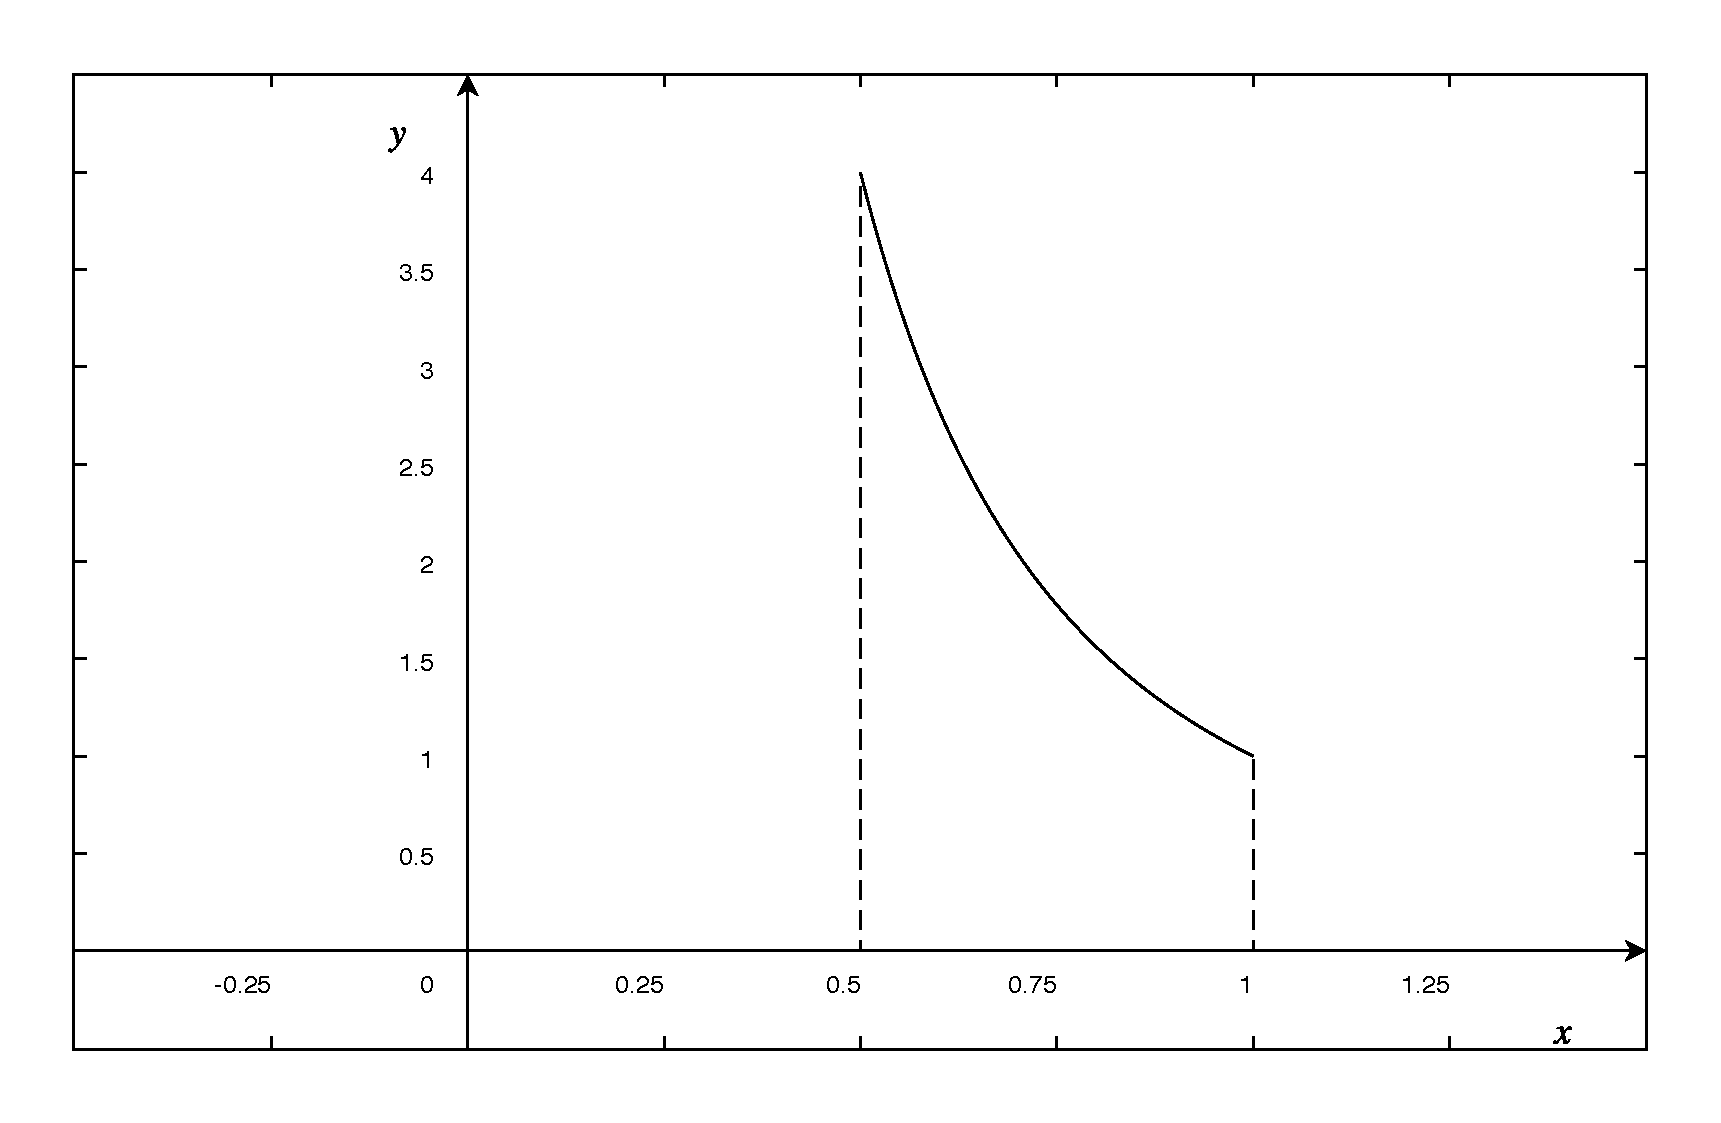
\includegraphics[width=0.5\textwidth]{Figures/Romeo_model_2.pdf}
  \end{figure}
\end{eg}
\begin{remark}[Bayes' rule variant]
  \[
    \mathbb{P}(\theta \vert x_1, x_2) = \dfrac{\mathbb{P}(x_2 \vert \theta, x_1) \mathbb{P}(\theta \vert x_1)}{\mathbb{P}(x_2 \vert x_1)}
  \]
\end{remark}
\begin{proof}
  \[
    \begin{aligned}
      f_{\Theta \vert X_1, X_2} \left(\theta \Big| \dfrac{1}{2}, \dfrac{1}{4}\right) &= \dfrac{f_{\Theta, X_1, X_2} \left(\theta, \dfrac{1}{2}, \dfrac{1}{4}\right)}{f_{X_1, X_2}\left(\dfrac{1}{2}, \dfrac{1}{4}\right)} \\
      &= \dfrac{f_{X_2 \vert \Theta, X_1} \left(\dfrac{1}{4} \Big| \theta, \dfrac{1}{2}\right) f_{\Theta, X_1}\left(\theta, \dfrac{1}{2}\right)}{f_{X_1, X_2}\left(\dfrac{1}{2}, \dfrac{1}{4}\right)} \\
      &= \dfrac{f_{X_2 \vert \Theta, X_1} \left(\dfrac{1}{4} \Big| \theta, \dfrac{1}{2}\right) f_{\Theta \vert X_1}\left(\theta \Big| \dfrac{1}{2}\right) f_{X_1} \left(\dfrac{1}{2}\right)}{f_{X_1, X_2}\left(\dfrac{1}{2}, \dfrac{1}{4}\right)} \\
      &= \dfrac{f_{X_2 \vert \Theta, X_1} \left(\dfrac{1}{4} \Big| \theta, \dfrac{1}{2}\right) f_{\Theta \vert X_1}\left(\theta \Big| \dfrac{1}{2}\right)}{f_{X_2 \vert X_1}\left(\dfrac{1}{4} \Big| \dfrac{1}{2}\right)} \\
    \end{aligned}
  \]
  Thus, 
  \[
    f_{\Theta \vert X_1, X_2} \left(\theta \Big| \dfrac{1}{2}, \dfrac{1}{4}\right) \propto f_{X_2 \vert \Theta, X_1} \left(\dfrac{1}{4} \Big| \theta, \dfrac{1}{2}\right) f_{\Theta \vert X_1}\left(\theta \Big| \dfrac{1}{2}\right)
  \]
\end{proof}